\documentclass{beamer}

\pdfmapfile{+sansmathaccent.map}


\mode<presentation>
{
	\usetheme{Warsaw} % or try Darmstadt, Madrid, Warsaw, Rochester, CambridgeUS, ...
	\usecolortheme{seahorse} % or try seahorse, beaver, crane, wolverine, ...
	\usefonttheme{serif}  % or try serif, structurebold, ...
	\setbeamertemplate{navigation symbols}{}
	\setbeamertemplate{caption}[numbered]
} 


%%%%%%%%%%%%%%%%%%%%%%%%%%%%
% itemize settings


%%%%%%%%%%%%%%%%%%%%%%%%%%%%
% itemize settings

\definecolor{myhotpink}{RGB}{255, 80, 200}
\definecolor{mywarmpink}{RGB}{255, 60, 160}
\definecolor{mylightpink}{RGB}{255, 80, 200}
\definecolor{mypink}{RGB}{255, 30, 80}
\definecolor{mydarkpink}{RGB}{155, 25, 60}

\definecolor{mypaleblue}{RGB}{240, 240, 255}
\definecolor{mylightblue}{RGB}{120, 150, 255}
\definecolor{myblue}{RGB}{90, 90, 255}
\definecolor{mygblue}{RGB}{70, 110, 240}
\definecolor{mydarkblue}{RGB}{0, 0, 180}
\definecolor{myblackblue}{RGB}{40, 40, 120}

\definecolor{myblackturquoise}{RGB}{5, 53, 60}
\definecolor{mydarkdarkturquoise}{RGB}{8, 93, 110}
\definecolor{mydarkturquoise}{RGB}{28, 143, 150}
\definecolor{mypaleturquoise}{RGB}{230, 255, 255}
\definecolor{myturquoise}{RGB}{48, 213, 200}

\definecolor{mygreen}{RGB}{0, 200, 0}
\definecolor{mydarkgreen}{RGB}{0, 120, 0}
\definecolor{mygreen2}{RGB}{245, 255, 230}

\definecolor{mygrey}{RGB}{120, 120, 120}
\definecolor{mypalegrey}{RGB}{160, 160, 160}
\definecolor{mydarkgrey}{RGB}{80, 80, 160}

\definecolor{mydarkred}{RGB}{160, 30, 30}
\definecolor{mylightred}{RGB}{255, 150, 150}
\definecolor{myred}{RGB}{200, 110, 110}
\definecolor{myblackred}{RGB}{120, 40, 40}


\definecolor{myblackmaroon}{RGB}{50, 0, 15}

\definecolor{mygreen}{RGB}{0, 200, 0}
\definecolor{mygreen2}{RGB}{205, 255, 200}

\definecolor{mydarkcolor}{RGB}{60, 25, 155}
\definecolor{mylightcolor}{RGB}{130, 180, 250}

\setbeamertemplate{itemize items}[default]

\setbeamertemplate{itemize item}{\color{myblackmaroon}$\blacksquare$}
\setbeamertemplate{itemize subitem}{\color{mydarkdarkturquoise}$\blacktriangleright$}
\setbeamertemplate{itemize subsubitem}{\color{mygray}$\blacksquare$}

\setbeamercolor{palette quaternary}{fg=white,bg=myblackmaroon}
\setbeamercolor{titlelike}{parent=palette quaternary}

\setbeamercolor{palette quaternary2}{fg=black,bg=mypaleblue}
\setbeamercolor{frametitle}{parent=palette quaternary2}

\setbeamerfont{frametitle}{size=\Large,series=\scshape}
\setbeamerfont{framesubtitle}{size=\normalsize,series=\upshape}





%%%%%%%%%%%%%%%%%%%%%%%%%%%%
% block settings

\setbeamercolor{block title}{bg=red!30,fg=black}

\setbeamercolor*{block title example}{bg=mygreen!40!white,fg=black}

\setbeamercolor*{block body example}{fg= black, bg= mygreen2}


%%%%%%%%%%%%%%%%%%%%%%%%%%%%
% URL settings
\hypersetup{
	colorlinks=true,
	linkcolor=blue,
	filecolor=blue,      
	urlcolor=blue,
}

%%%%%%%%%%%%%%%%%%%%%%%%%%

\renewcommand{\familydefault}{\rmdefault}

\usepackage{amsmath}
\usepackage{mathtools}

\usepackage{subcaption}

\usepackage{qrcode}

\DeclareMathOperator*{\argmin}{arg\,min}
\newcommand{\bo}[1] {\mathbf{#1}}

\newcommand{\R}{\mathbb{R}} 
\newcommand{\T}{^\top}     



\newcommand{\mydate}{Fall 2023}

\newcommand{\mygit}{\textcolor{blue}{\href{https://github.com/SergeiSa/Mechatronics-2023}{github.com/SergeiSa/Mechatronics-2023}}}

\newcommand{\myqr}{ \textcolor{black}{\qrcode[height=1.5in]{https://github.com/SergeiSa/Mechatronics-2023}}
}

\newcommand{\myqrframe}{
	\begin{frame}
		\centerline{Lecture slides are available via Github, links are on Moodle}
		\bigskip
		\centerline{You can help improve these slides at:}
		\centerline{\mygit}
		\bigskip
		\myqr
	\end{frame}
}


\newcommand{\bref}[2] {\textcolor{blue}{\href{#1}{#2}}}

%%%%%%%%%%%%%%%%%%%%%%%%%%%%
% code settings

\usepackage{listings}
\usepackage{color}
% \definecolor{mygreen}{rgb}{0,0.6,0}
% \definecolor{mygray}{rgb}{0.5,0.5,0.5}
\definecolor{mymauve}{rgb}{0.58,0,0.82}
\lstset{ 
	backgroundcolor=\color{white},   % choose the background color; you must add \usepackage{color} or \usepackage{xcolor}; should come as last argument
	basicstyle=\footnotesize,        % the size of the fonts that are used for the code
	breakatwhitespace=false,         % sets if automatic breaks should only happen at whitespace
	breaklines=true,                 % sets automatic line breaking
	captionpos=b,                    % sets the caption-position to bottom
	commentstyle=\color{mygreen},    % comment style
	deletekeywords={...},            % if you want to delete keywords from the given language
	escapeinside={\%*}{*)},          % if you want to add LaTeX within your code
	extendedchars=true,              % lets you use non-ASCII characters; for 8-bits encodings only, does not work with UTF-8
	firstnumber=0000,                % start line enumeration with line 0000
	frame=single,	                   % adds a frame around the code
	keepspaces=true,                 % keeps spaces in text, useful for keeping indentation of code (possibly needs columns=flexible)
	keywordstyle=\color{blue},       % keyword style
	language=Octave,                 % the language of the code
	morekeywords={*,...},            % if you want to add more keywords to the set
	numbers=left,                    % where to put the line-numbers; possible values are (none, left, right)
	numbersep=5pt,                   % how far the line-numbers are from the code
	numberstyle=\tiny\color{mygray}, % the style that is used for the line-numbers
	rulecolor=\color{black},         % if not set, the frame-color may be changed on line-breaks within not-black text (e.g. comments (green here))
	showspaces=false,                % show spaces everywhere adding particular underscores; it overrides 'showstringspaces'
	showstringspaces=false,          % underline spaces within strings only
	showtabs=false,                  % show tabs within strings adding particular underscores
	stepnumber=2,                    % the step between two line-numbers. If it's 1, each line will be numbered
	stringstyle=\color{mymauve},     % string literal style
	tabsize=2,	                   % sets default tabsize to 2 spaces
	title=\lstname                   % show the filename of files included with \lstinputlisting; also try caption instead of title
}


%%%%%%%%%%%%%%%%%%%%%%%%%%%%
% URL settings
\hypersetup{
	colorlinks=false,
	linkcolor=blue,
	filecolor=blue,      
	urlcolor=blue,
}

%%%%%%%%%%%%%%%%%%%%%%%%%%

%%%%%%%%%%%%%%%%%%%%%%%%%%%%
% tikz settings

\usepackage{tikz}
\tikzset{every picture/.style={line width=0.75pt}}


\title{MPC, Whole-body impulse control}
\subtitle{Contact-aware Control, Lecture 11}
\author{by Sergei Savin}
\centering
\date{\mydate}



\begin{document}
\maketitle


\begin{frame}{Content}

\begin{itemize}
\item Single rigid body model
\item Bilinearity
\item Linearizing rotation
\item Model-predictive control
\item Whole-body impulse control
\item Quadruped control - big picture
\end{itemize}

\end{frame}




\begin{frame}{Single rigid body model, 1}
	% \framesubtitle{Parameter estimation}
	\begin{flushleft}
		
		One of possible simplified models of walking robots is a single rigid body model. There are two ways to think about it:
		
		\begin{itemize}
			\item A robot consists of a body and legs. We assume that the mass and the inertia of the legs is much less than that of the body. This allows us to ignore the legs of the robot and model it as a body with reaction forces acting on it.
			
			\item Instead of modeling the robot using Lagrangian mechanics, we use a simplified model - we find a single rigid body model that describes the actual robot in the best possible way.
		\end{itemize}
		
	\end{flushleft}
\end{frame}



\begin{frame}{Single rigid body model, 2}
	% \framesubtitle{Parameter estimation}
	\begin{flushleft}
		
		Single rigid body model can be described as:
		
		\begin{align}
			m \ddot{\bo{p}} &= \sum \bo{f}_i + \bo{g} 
			\\
			\frac{d}{dt}(\bo{I}\omega) &= \sum (\bo{r}_i \times \bo{f}_i)
		\end{align}
		%
		where $\bo{p}$ is the position of the center of mass of the body, $m$ and $\bo{I}$ is its mass and inertia, $\omega$ is its angular velocity, $\bo{f}_i$ are reaction forces, $\bo{r}_i$ are contact position and $\bo{g}$ is gravitational force.
		
	\end{flushleft}
\end{frame}



\begin{frame}{Bilinearity, 1}
	% \framesubtitle{Parameter estimation}
	\begin{flushleft}
		
		Equation $m \ddot{\bo{p}} = \sum \bo{f}_i + \bo{g} $ shows a linear relation between acceleration $\ddot{\bo{p}}$ and reaction forces $\bo{f}_i$. Linear equations of this type can be used as a constraint in convex optimization problems (COP). COP usually allow linear equality constraints, but not other types of equality constraints. 
		
		\bigskip
		
		Note that constraint $\frac{d}{dt}(\bo{I}\omega) = \sum (\bo{r}_i \times \bo{f}_i)$ is bilinear in position variables $\bo{r}_i$ and and reaction forces $\bo{f}_i$. This reflects the fact that torques depend linearly both on the force and point of application of this force. To use such constraint in COP, one of the two components has to be assumed to be constant - either point of application or the reaction force.
		
	\end{flushleft}
\end{frame}



\begin{frame}{Bilinearity, 2}
	% \framesubtitle{Parameter estimation}
	\begin{flushleft}
		
		Bilinearity introduced by torques has a few important consequences:
		
		\begin{itemize}
			\item For trajectory planning problem (TPP) in full coordinates (or even when using SRB model) this means that the problem is not convex; TPP will be solved with non-linear solvers.
			
			\item For problems that need to be solved with convex solvers (such as MPC problems) the positions of contact points $\bo{r}_i$ is fixed, making r.h.s. of the equation $\frac{d}{dt}(\bo{I}\omega) = \sum (\bo{r}_i \times \bo{f}_i)$ linear in decision variables.
		\end{itemize}
		
	\end{flushleft}
\end{frame}



\begin{frame}{Linearizing rotation}
	% \framesubtitle{Parameter estimation}
	\begin{flushleft}
		
		To linearize SRB dynamics we need to further introduce new variables and simplifications. Let $\Theta \in \R^3$ be encoding of robot orientation. Then we can simplify dynamics as:
		
		\begin{align}
			\dot \Theta &= \bo{R}\omega 
			\\
			\bo{I}_\mathcal{G} \dot \omega &= \sum ( [\bo{r}_i]_\times \bo{f}_i)
		\end{align}
		
		Where $\bo{R}$ is orientation matrix, $\bo{I}_\mathcal{G} = \bo{R} \bo{I}_\mathcal{B} \bo{R}\T $ is inertial tensor in the global frame, and $\bo{I}_\mathcal{B}$ - inertial tensor in the local frame.
		
	\end{flushleft}
\end{frame}


\begin{frame}{Model-predictive control, 1}
	% \framesubtitle{Parameter estimation}
	\begin{flushleft}
		
		Assuming discretization time step $\Delta t$, we get the following simplified discrete dynamics:
		
		\begin{equation}
			\bo{x}_{k+1} = \bo{A}_k \bo{x}_k + \bo{B}_k \hat{\bo{f}}_k + \hat{\bo{g}}
		\end{equation}
		%
		where: 
		
		$\bo{x}= \begin{bmatrix}
			\Theta\T & \bo{p}\T & \dot \Theta\T & \dot{\bo{p}}\T
		\end{bmatrix}\T$,
		%
		$ \hat{\bo{f}}= \begin{bmatrix}
			\bo{f}_1\T & ... & \bo{f}_n\T
		\end{bmatrix}\T$,
	
		$ \hat{\bo{g}}= \begin{bmatrix}
		\bo{0}_{3 \time 1}  & \bo{0}_{3 \time 1} & \bo{0}_{3 \time 1}  & \bo{g}\T
		\end{bmatrix}\T$,
	
		$\bo{A}= \begin{bmatrix}
		\bo{1}_{3 \time 3}  & \bo{0}_{3 \time 3} & \bo{R}\Delta t  & \bo{0}_{3 \time 3}
		\\
		\bo{0}_{3 \time 3} & \bo{1}_{3 \time 3}  & \bo{0}_{3 \time 3} & \bo{1}_{3 \time 3} \Delta t 
		\\
		\bo{0}_{3 \time 3} & \bo{0}_{3 \time 3} & \bo{1}_{3 \time 3}  & \bo{0}_{3 \time 3} 
		\\
		\bo{0}_{3 \time 3} & \bo{0}_{3 \time 3} & \bo{0}_{3 \time 3} & \bo{1}_{3 \time 3}
		\end{bmatrix}$, 
	%
		$\bo{B}= \begin{bmatrix}
			\bo{0}_{3 \time 3}  & ...  & \bo{0}_{3 \time 3}
			\\
			\bo{0}_{3 \time 3} & ... & \bo{0}_{3 \time 3}
			\\
			\bo{I}_\mathcal{G}^{-1} [\bo{r}_1]_\times \Delta t  & ...  & \bo{I}_\mathcal{G}^{-1} [\bo{r}_n]_\times \Delta t 
			\\
			\bo{1}_{3 \time 3} \Delta t / m & ... & \bo{1}_{3 \time 3} \Delta t / m
		\end{bmatrix}$
		
	\end{flushleft}
\end{frame}


\begin{frame}{Model-predictive control, 2}
	% \framesubtitle{Parameter estimation}
	\begin{flushleft}
		
		Parameterizing reaction forces as $\bo{f}_j = \begin{bmatrix}
			f_{j, x} & f_{j, y} & f_{j, z}
		\end{bmatrix}\T$ 
		we can use a simple linear approximation of a friction cone:
		
		\begin{align}
			| f_{j, x} | \leq  \mu f_{j, z} 
			\\
			| f_{j, y} | \leq \mu f_{j, z} 
		\end{align}
	
		To simplify notation we can designate friction cone constraint as $\hat{\bo{f}} \in \mathcal{C}$.
	
		
		
	\end{flushleft}
\end{frame}



\begin{frame}{Model-predictive control, 3}
	% \framesubtitle{Parameter estimation}
	\begin{flushleft}
		
		Finally, we formulate MPC as a quadratic program:
		
		\begin{align*}
			\underset{\bo{x}_{k+1}, \hat{\bo{f}}_k}{\text{minimize}}
			 & \ \ \sum || \bo{x}_{k+1} - \bo{x}_{k+1}^\text{ref} ||_\bo{Q} +
			         \sum || \hat{\bo{f}}_k ||_\bo{R},
			\\
			\text{subject to:} & \ \ 
			\bo{x}_{k+1} = \bo{A}_k \bo{x}_k + \bo{B}_k \hat{\bo{f}}_k + \hat{\bo{g}},
			\\
			& \ \ \hat{\bo{f}} \in \mathcal{C}.
		\end{align*}
		%
		where $|| \bo{x} ||_\bo{Q} = \sqrt{\bo{x}\T \bo{Q} \bo{x}} $ - weighted norm, $\bo{Q}$, $\bo{R}$ - weight matrices and $\bo{x}_{k+1}^\text{ref}$ - reference trajectory.
		
		\bigskip
		
		This MPC can be run at 40 Hz. This gives us desired reaction forces, which we can use to compute joint torques.
		
	\end{flushleft}
\end{frame}




\begin{frame}{Whole-body impulse control (WBIC), 1}
	% \framesubtitle{Parameter estimation}
	\begin{flushleft}
		
		We can write manipulator dynamics in the following way:
		
		\begin{equation}
			\bo{H}
			\begin{bmatrix}
				\ddot{\bo{q}}_F \\ \ddot{\bo{q}}_J 
			\end{bmatrix}
		+ \bo{C} \dot{\bo{q}} + \bo{g}
		=
		\begin{bmatrix}
			\bo{0}_6 \\ \tau
		\end{bmatrix}
		+
		\bo{J}_c\T \lambda 
		\end{equation}
		%
		where $\bo{q}_F$ - floating-base coordinates and $\bo{q}_J$ - joint-space coordinates, $\bo{H}$ - generalized inertia matrix, $\bo{C}$ - Coriolis inertial force matrix, $\bo{g}$ - generalized gravitational force, $\tau$ - joint torques, $\bo{J}_c$ - constraint Jacobian and $\lambda$ - reaction forces.
		
		
	\end{flushleft}
\end{frame}



\begin{frame}{Whole-body impulse control (WBIC), 2}
	% \framesubtitle{Parameter estimation}
	\begin{flushleft}
		
		In order to compute joint torques, we can formulate the following quadratic problem:
		
		\begin{align*}
			\underset{\delta_a, \delta_f}{\text{minimize}}
			& \ \ \delta_a\T \bo{Q} \delta_a + \delta_f\T \bo{R} \delta_f,
			\\
			\text{subject to:} & \ \ 
			\bo{S} ( \bo{H} \ddot{\bo{q}}  + \bo{C} \dot{\bo{q}} + \bo{g} ) =
			\bo{S}\bo{J}_c\T (\bo{f}_\text{MPC} +  \delta_f) ,
			\\
			& \ \ \ddot{\bo{q}} = \ddot{\bo{q}}_\text{des} + 
			\begin{bmatrix}
				 \delta_a \\ \bo{0}
			\end{bmatrix}
			\\
			& \ \ \bo{f}_\text{MPC} +  \delta_f \in \mathcal{C}.
		\end{align*}
		%
		where $\bo{S} = \begin{bmatrix}
			\bo{1}_{6 \times 6} & 0
		\end{bmatrix}$ is  a floating-base selection matrix, $\bo{f}_\text{MPC}$ is a reference for the reaction force found from solving MPC and $\ddot{\bo{q}}_\text{des}$ is the desired acceleration found from inverse kinematics.
		
	\end{flushleft}
\end{frame}





\begin{frame}{Whole-body impulse control (WBIC), 3}
	% \framesubtitle{Parameter estimation}
	\begin{flushleft}
		
		This controller can be solved at a rate of 500 Hz. Result of solving this QP is the value for decision variables $\delta_a, \delta_f$ which allow us to compute the acceleration and reaction forces:
		
		\begin{align}
			\ddot{\bo{q}} = \ddot{\bo{q}}_\text{des} + 
			\begin{bmatrix}
				\delta_a \\ \bo{0}
			\end{bmatrix} 
		\\
		\lambda  = \bo{f}_\text{MPC} +  \delta_f
		\end{align}
		
		Knowing both we can compute the torques using manipulator equations:
		
		\begin{equation}
			\begin{bmatrix}
				\bo{0}_6 \\ \tau
			\end{bmatrix}
		=
		\bo{H}\ddot{\bo{q}}
		+ \bo{C} \dot{\bo{q}} + \bo{g}
			-
			\bo{J}_c\T \lambda 
		\end{equation}
		
	\end{flushleft}
\end{frame}




\begin{frame}{Quadruped control - big picture, 1}
	% \framesubtitle{Parameter estimation}
	\begin{flushleft}
		
		% TODO: \usepackage{graphicx} required
		\begin{figure}
			\centering
			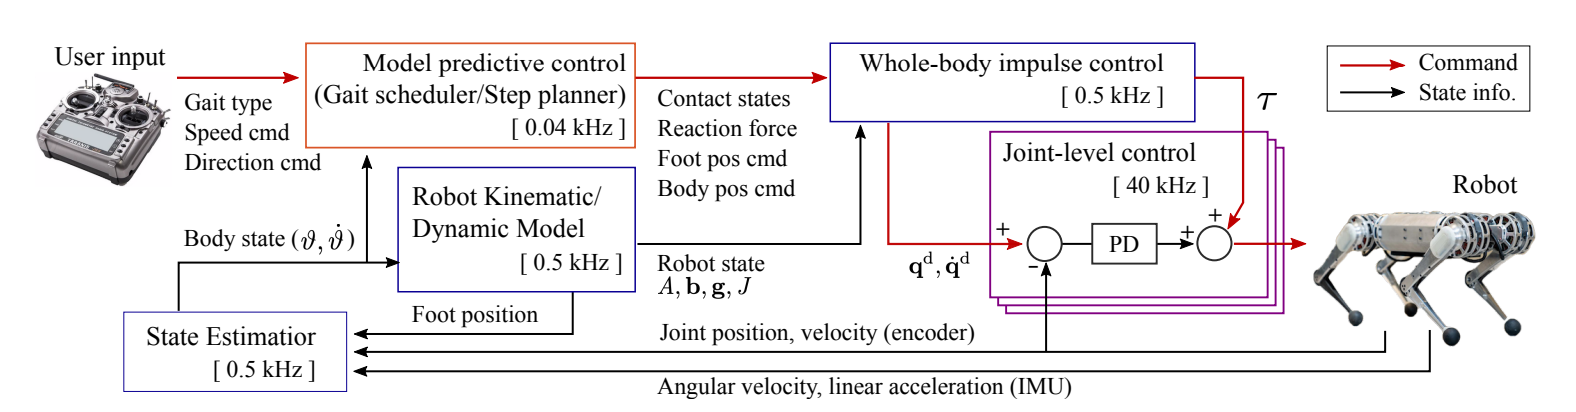
\includegraphics[width=1.1\linewidth]{ControlSystemKim_1}
			\caption{Control scheme proposed by Kim et al.}
			\label{fig:controlsystemkim1}
		\end{figure}
		
	\end{flushleft}
\end{frame}



\begin{frame}{Quadruped control - big picture, 2}
	% \framesubtitle{Parameter estimation}
	\begin{flushleft}
		
		% TODO: \usepackage{graphicx} required
		\begin{figure}
			\centering
			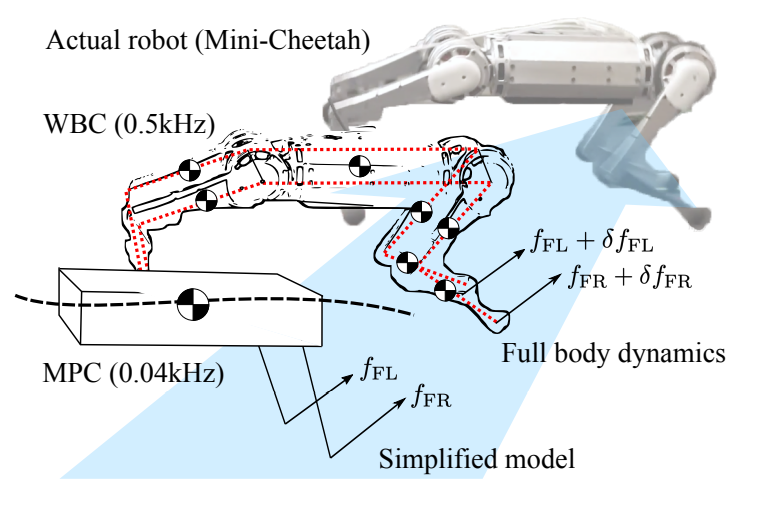
\includegraphics[width=0.8\linewidth]{ControlSystemKim_2}
			\caption{Sub-levels of the control system, as proposed by Kim et al.}
			\label{fig:controlsystemkim2}
		\end{figure}
		
		
	\end{flushleft}
\end{frame}




\begin{frame}{Read more}
	\begin{itemize}
		\item Kim, D., Di Carlo, J., Katz, B., Bledt, G. and Kim, S., 2019. Highly dynamic quadruped locomotion via whole-body impulse control and model predictive control.  \bref{https://arxiv.org/abs/1909.06586}{arXiv:1909.06586}
		
	\end{itemize}
\end{frame}



\myqrframe

\end{document}
